% ITEX root = ../Thesis.tex
\subsection{Wrangled data and starting parameters}
\begin{wrapfigure}{r}{0.4\textwidth}
    \begin{center}
        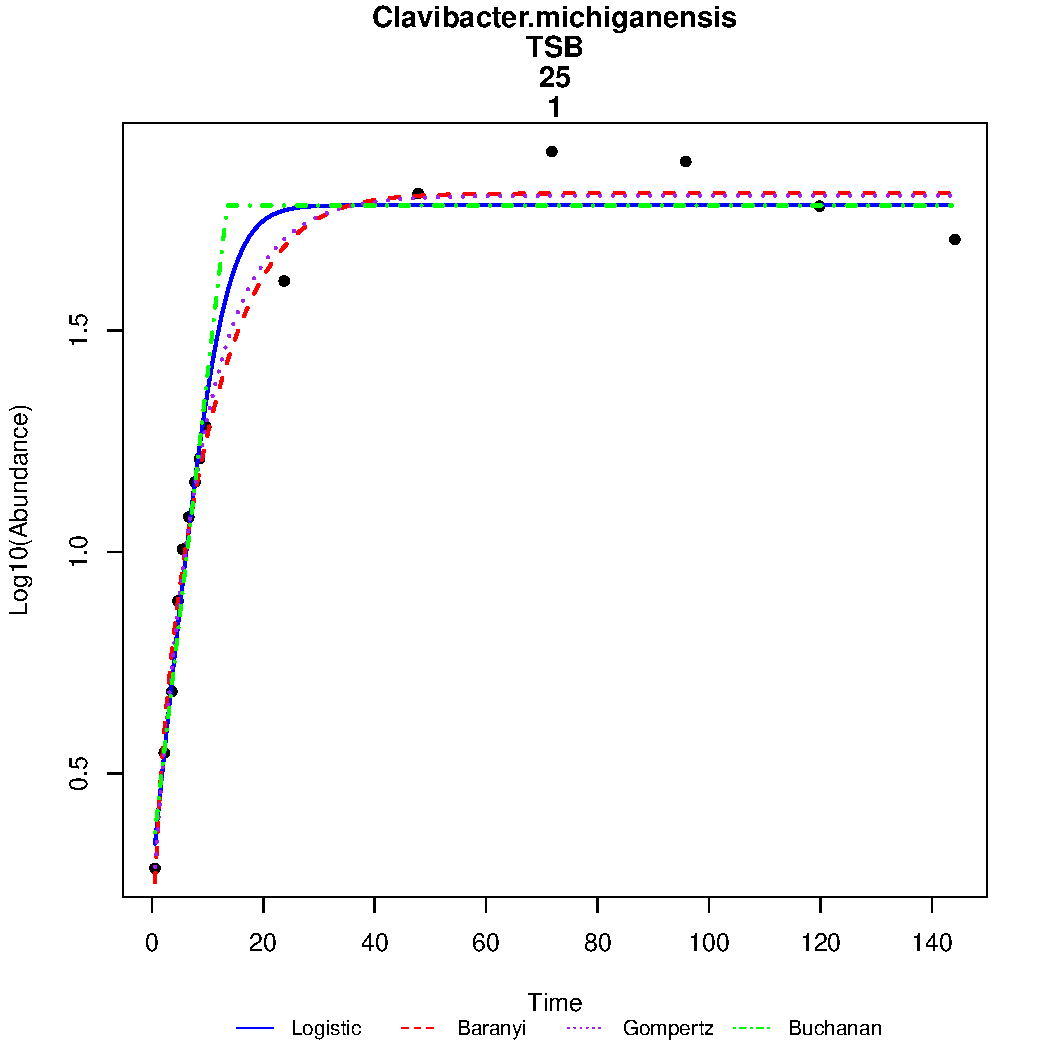
\includegraphics[width=0.48\textwidth]{../Results/Cmichiganensis25_fit.pdf}
    \end{center}
    \caption{Clavibacter michiganensis model fit showing the death phase}
    \label{fig:Clavibacter michiganensis}
\end{wrapfigure}

When visualising the data, the common log of the abundance produced either a slight sigmoidal functions or log distribution, which is expected. Distribution of the data sets were not consistent as some plots revealed no pattern, having a random distribution of points along the axis, unable to derive starting parameter values and overall fit the models. Furthermore, some of the data sets revealed a decline once the asymptotic value has been reached. This is the death phase which is ignored in the model fitting process (Zwietering et al., 1990).

Getting all required starting parameters is necessary for the model fittings to be produced. Despite not all the data sets followed a sigmoidal or log distribution, positive $r_{max}$ and  $t_{lag}$ values were still derived from all the data sets. Although the Logistic model only requires three of the starting parameters, the growth rate parameter is the determining factor of all the models fitting. Starting population ($N_0$) and carrying capacity ($N_{max}$) are easily derived from the data sets however, growth rate and time lag are mathematical derivations thus have the possibility of having NA values depending on the distribution of data points. The growth rate coefficient represents the max slope between points, which is the derivative along the inflection point. While the $t_{lag}$ requires the y-intercept of $r_max$ slope as well as the actual slope value to derive it.

\subsection{Model fitting}
\begin{figure*}[h!]
    \centering
    \begin{subfigure}[h]{0.4\textwidth}
        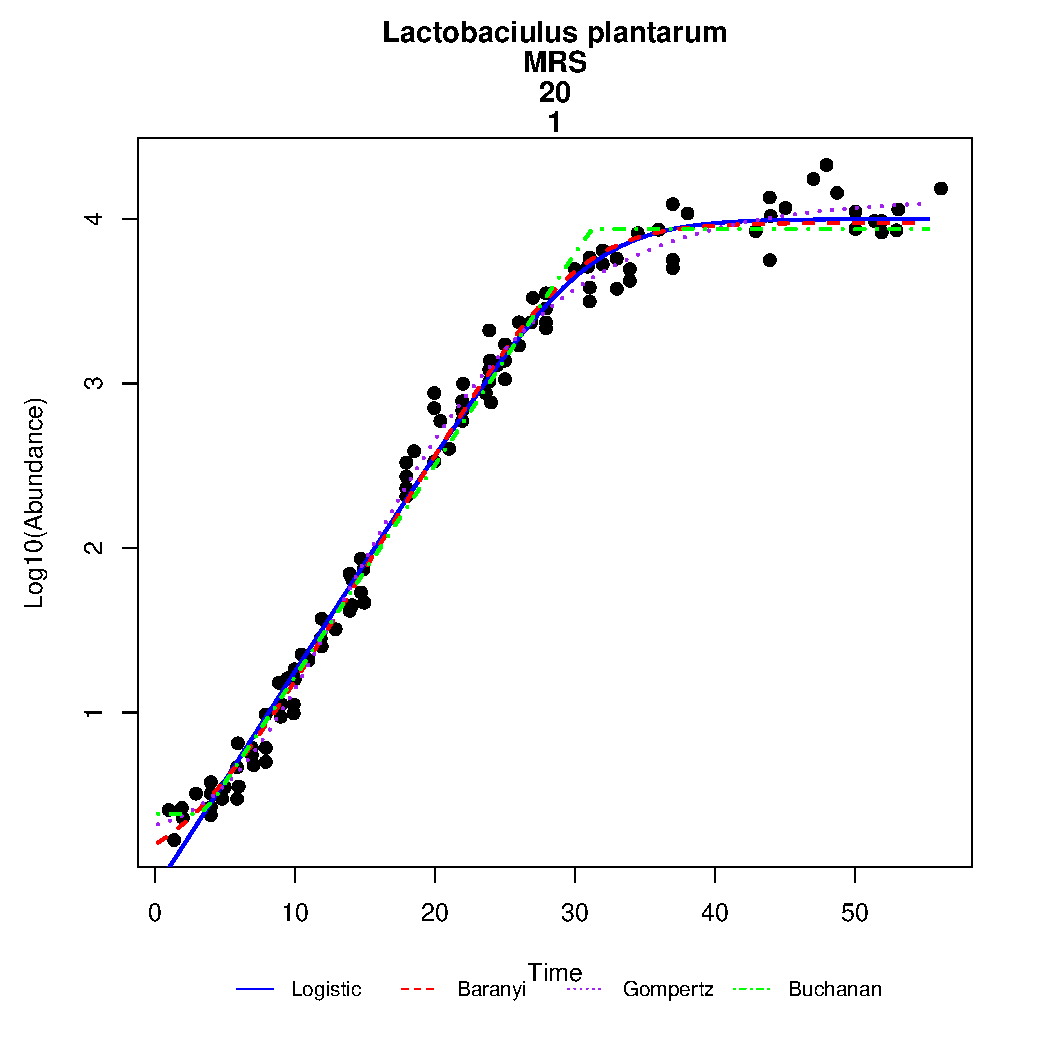
\includegraphics[width=\textwidth]{../Results/Lplantarum_fit.pdf}
        \caption{Figure 3.1: Lactobaciulus plantarum model fit}
        \label{fig:Lactobaciulus plantarum}
    \end{subfigure}
    \hfill
    \begin{subfigure}[h]{0.4\textwidth}
        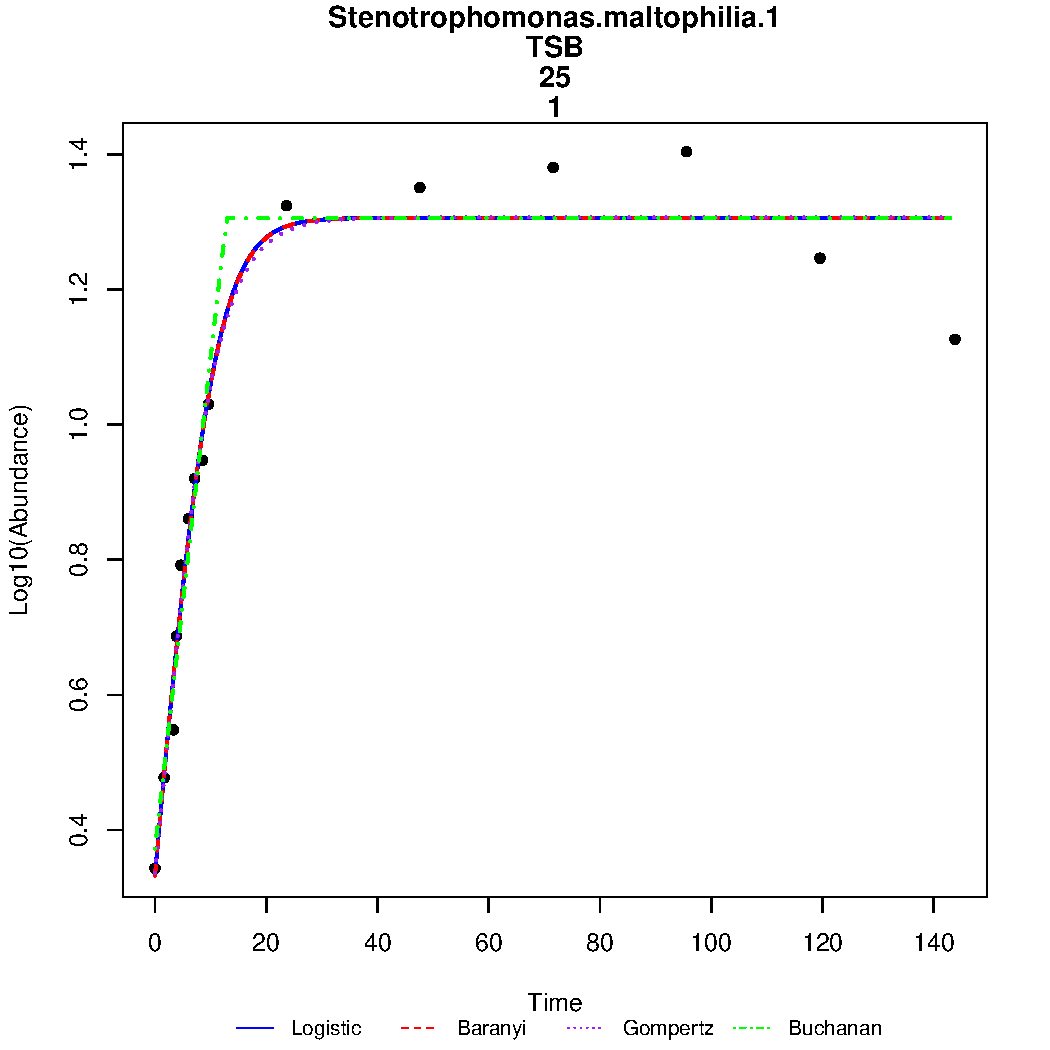
\includegraphics[width=\textwidth]{../Results/Smaltophilia25_fit.pdf}
        \caption{Figure 3.2: Stenotrophomonas maltophilia model fit}
        \label{fig:Stenotrophomonas maltophilia}
    \end{subfigure}
\end{figure*}

All four models were nested upon each other, utilising similar parameters. The Logistic model is derived from external limiting factors including resource and density. These external factors play limit the exponential growth of the population, hence producing the sigmoidal shape where it reaches an asymptotic value known as the carrying capacity \cite{webb1986logistic}. The Baranyi model is a differential model which accounts biological factors of individual microbial growth. It takes into account environmental variation and the physiological limiting factors, specifically the limits in the rate of biochemical reactions within the microbe \cite{buchanan1997simple, grijspeerdt1999estimating}. The Buchanan model is a simplified version of the Gompertz model and Baranyi model, which accounts for biological variability, considering individual physiological factors and population factors such as adaptation at each of the growth phases to produce a three-phase linear model \cite{buchanan1997simple} et al., 1997).

Overall, the results show that the Gompertz model was the most robust model, having the greatest number of goodness of fit. In other words, for the provided data set, it is the best model to describe the population dynamics of microbial growth over time. This is not surprising as it is a primary level model, which only describes change population over time \cite{grijspeerdt1999estimating}. The Gompertz model is mathematical derivations to form the sigmoidal relationship \cite{buchanan1997simple} et al., 1997). Despite its parameters, it is an empirical derivation not accounting for any biological processes. The robustness of the model is from the parameters. The parameters account for shape or curvature of the fit, and location along the axis, allowing the model to shift the fit along the x-axis or y-axis and maintain its overall shape \cite{tjorve2017use}. Furthermore, similar to the method of deriving the growth rate from the data sets, the growth rate in the Gompertz model is derived along the inflection point.

\subsection{AIC}

Best fitting model was determined through the AIC values produced. From the results, the Gompertz model was the most robust, having the most number of fits. This is due to the derivation and robustness of the parameters, as well as the flexibility of the model \cite{tjorve2017use}. Depending on the data set, the AIC values produced negative or positive ranges of values, and the best model fit was the model that produced the minimum value relative to the other fits. The AIC values here shows that Gompertz model most likely explains the data sets however, cannot explain how “true” realism, since we are only comparing relatively between the four models. AIC  considers the trade-off between model complexity and fit \cite{vrieze2012model}. AIC does favour more complex models as from the formula, the $-2 \cdot \mathcal{L}$ is decreased (Posada and Buckley, 2004). This is why the Gompertz model performed well as it contains four parameters. The extra parameter in addition with the flexibility of the model itself makes it a robust fit.

\newpage

\subsection{Temperature and Growth Rate Correlation}
\begin{table}[h!]
\centering
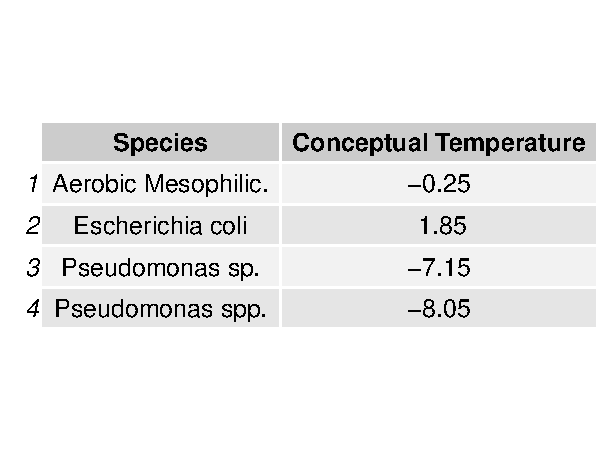
\includegraphics[scale=0.60]{../Results/Species_ConceptualTemp.pdf} \caption{Provided conceptual temperatures of species in data set} \label{tab:Conceptual Temperature}
\end{table}

\begin{wrapfigure}{r}{0.3\textwidth}
    \begin{center}
        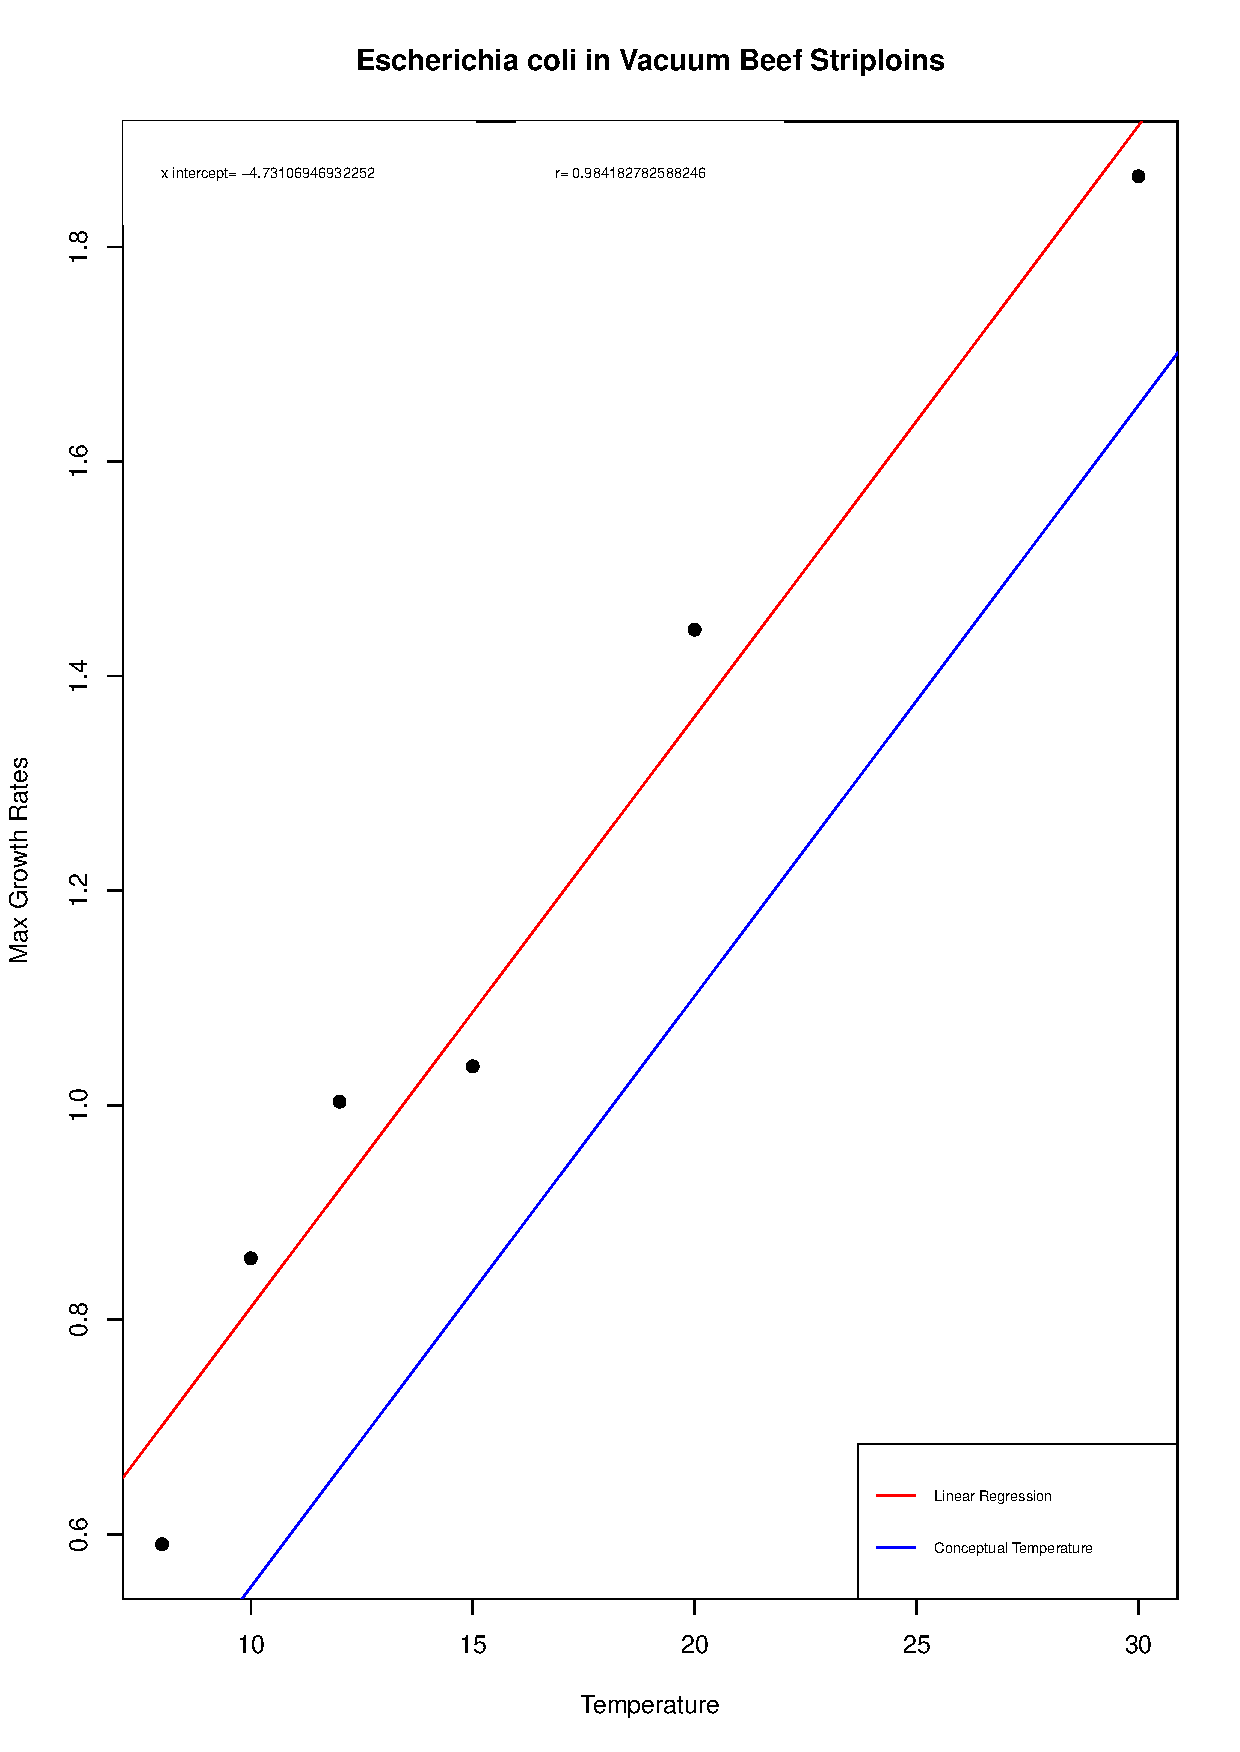
\includegraphics[width=0.40\textwidth]{../Results/Ecoli_r_temp.pdf}
    \end{center}
    \caption{Escherichia Coli recorded growth rates plotted against temperature}
    \label{fig:E.coli correlation}
\end{wrapfigure}

Using the species with recordings of conceptual temperature, the plots show that there is a strong positive correlation between growth rate and temperature. A linear regression analysis was done and also fitting the the formula given from \textit{Ratkowsky et al.} Unlike the original paper, the distribution of points were not as linear but this is likely due to data collection methods from the data provided as well as the temeperature tolerances of the different species. Using the linear regression analysis, x-intercept values were calculated to see if they coincide with conceptual temperatures \cite{ratkowsky1982relationship}. The x-intercepts vary from the conceptual temperatures provided from the paper. From the plot, aside from the \textit{Aerobic Mesophilic} in \textit{Cooked Chicken Breast}, the Conceptual Temperature model did not align with the data well.

Furthermore looking at the regression analysis, if we use a significance value of 0.05, using fisher’s method for independent test statistics, which takes the logarithm of the p-values \cite[p.103]{fisher1992statistical}. The resulting p-value is much less than the significant level. This means that the slopes are statistically significant, not random and support the positive correlation between temperature and growth rate. Only five species were investigated but further analysis can be done as conceptual temperature values are collected for the other species in the provided data. Overall, the results show that temperature and growth rate are positively correlated.
